\frame{
  \frametitle{Estado del Arte}
\begin{block}{Recordemos...}

 \begin{itemize}[<+-| alert@+>]
        \item Interoperabilidad.
        \item Integración.
        \item SOA.
        \item Semántica+SOA.
\end{itemize}
\end{block}

}

\subsection{Interoperabilidad}

\frame{
  \frametitle{Interoperabilidad} 
\begin{block}{Objetivos}

 \begin{itemize}
  \item  Mejorar la comunicación entre aplicaciones.
  \item  Homogeneizar un entorno heterogéneo en cuanto a formato de datos y
protocolos de comunicaciones.
\item Aplicar estándares acordados de forma comunitaria.
\item Agilizar los procesos de desarrollo y de mantenimiento.
\item Facilitar los entornos de pruebas.
\item Reutilizar lógica de negocio.
\end{itemize}
\end{block}

}

\frame{
  \frametitle{Interoperabilidad} 
\begin{block}{Tipos}

 \begin{enumerate}[<+->]
\item Sintáctica. Intercambio de datos en un formato determinado y bajo
unos ciertos protocolos de comunicaciones. Por ejemplo: SOAP+XML.

\item Semántica. Sintáctica+interpretación automática. Por ejemplo:
descubrimiento, selección, etc.
\end{enumerate}
\end{block}

}


\frame{
  \frametitle{Interoperabilidad} 
\begin{block}{La conseguimos si...}

 \begin{itemize}


\item Usamos estándares. Por ejemplo: XBRL (acuerdo en un sector).

\item Tecnología común de comunicaciones.Por ejemplo: SOAP 1.1.

\item Implementaciones usando estándares. Esfuerzo para trabajar con los datos
en el formato estándar (importar y exportar).

\end{itemize}
\end{block}

}


\frame{
  \frametitle{Interoperabilidad} 
\begin{block}{en SOA...}

 \begin{itemize}

\item Uso de estándares. Por ejemplo: BPEL~\cite{IBMBPEL2007}.


\item Recursos que proporciona WS-I (\url{http://www.ws-i.org/}).


\item Uso de SOAP 1.1 sobre REST.


\item Descripciones precisas y mecanizables de los servicios web
utilizando el lenguaje WSDL 1.1-2.0. 


\item Capacidades de SOAP y WSDL para la gestión y
recuperación de errores. 

\item Servicios como parte de una arquitectura. Procesos complejos se fragmentan
en servicios más sencillos orquestados.

\item Compromiso de mantener estable el API de los servicios web.

\item Diseño del interfaz por contrato y dirigido por datos.

\end{itemize}
\end{block}

}


\frame{
  \frametitle{Interoperabilidad} 
\begin{exampleblock}{y si unimos semántica...}

 \begin{itemize}
\item  Modelo de datos y formato estándar.
\item  El contenido es usable desde que está disponible.
\item  Es un formato procesable por las máquinas.
\item La información existente es fácilmente representable.
\item Flexibilidad en la representación de la información.
\end{itemize}
\end{exampleblock}

}

\frame{
  \frametitle{Interoperabilidad} 

\begin{figure}[htb]
\centering
	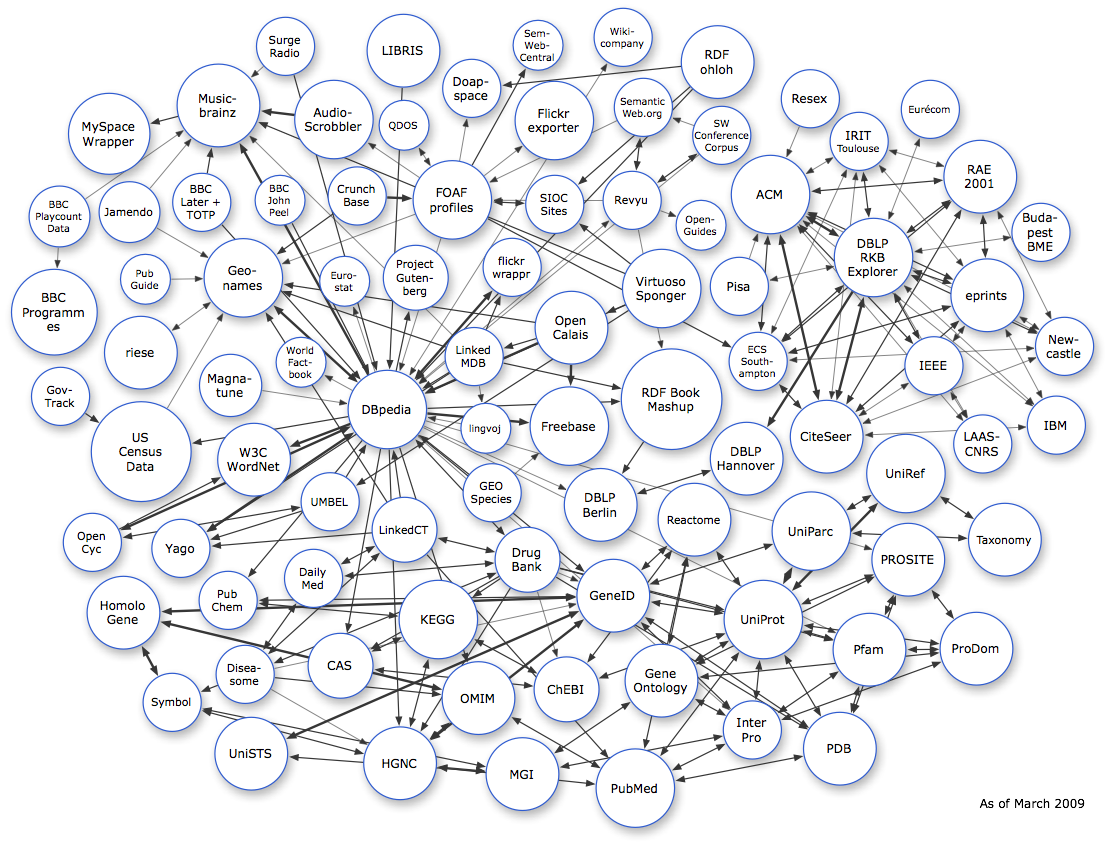
\includegraphics[width=8cm]{images/linked-data}
\caption{Nube de Linked Data.}
\end{figure}

}



\subsection{Integración}

\frame{
  \frametitle{Integración} 

\begin{block}{Objetivos}

 \begin{itemize}
 \item Aunar la estrategia corporativa para que los desarrollos utilicen una
infraestructura de comunicación común.
 \item Mejorar la fiabilidad de las comunicaciones.
 \item Disponer de una estructura sin mantenimiento especial.
\item Mantener compatibilidad hacia atrás.
\item Crear una infraestructura escalable.
\item Mejorar el mantenimiento, control y gobierno de la infraestructura.
\end{itemize}
\end{block}
}

\frame{
  \frametitle{Integración} 
\begin{block}{Tipos}

 \begin{enumerate}[<+->]


\item Datos. Por ejemplo: BB.DD.

 \item Métodos u operaciones. Integración A2A (\textbf{A}pplication 2
\textbf{A}pplication). Por ejemplo: como EJB, CORBA, RMI o DCOM. 

 \item Interfaz de usuario. Estandarización de interfaces de usuarios. Por
ejemplo: Gestores de contenidos, JSF, Portlets.

\item Proceso de negocio. Proceso como unidad mínima a combinar. Integración B2B
(\textbf{B}usiness 2 \textbf{B}usiness). Por ejemplo: WSDL, SOAP o BPEL y
productos asociados (OrableBPEL, JBPM, Apache ODE, AXIS, etc.).

\end{enumerate}
\end{block}

}



\frame{
  \frametitle{Integración} 
\begin{block}{en SOA...}
 \textit{Enterprise Service Bus (ESB)}~\cite{esb}.
\end{block}
(lo veremos en la siguiente sección).
}

\subsection{SOA}

\frame{
  \frametitle{SOA} 

\begin{figure}[htb]
\centering
	
\includegraphics[width=6cm]{images/puzzle-lg}
\caption{SOA solución integrada e interoperable.}
\end{figure}

}


\frame{
  \frametitle{SOA} 
\begin{block}{Tres elementos constitutivos~\cite{SoaInPractice}}

 \begin{enumerate}[<+->]

 \item Servicios.
 \item Infraestructura.
 \item Políticas.

\end{enumerate}
\end{block}

}




\frame{
  \frametitle{Servicios} 
\begin{exampleblock}{Servicios}<1->
Entidades abstractas que ejecutan cierta lógica de negocio y que son
independientes de la implementación.
\end{exampleblock}

\begin{block}{Visión}<2->
Supone un paso en la ejecución de un proceso mayor, visión compartida
con el ``Business Process Management''~\cite{bpm}.
\end{block}

}



\frame{
  \frametitle{Servicios} 
\begin{exampleblock}{Implementación}
Un servicio web es un recurso accesible a través de los protocolos de Internet y
que proporciona una funcionalidad determinada de acuerdo a unas especificaciones
y protocolos particulares. Su interfaz expone: operaciones  disponibles,  tipos
de mensajes a intercambiar durante la interacción con el servicio y localización
física (dirección + puerto). 
\end{exampleblock}

}


\frame{
  \frametitle{Servicios} 

\begin{figure}[htb]
\centering
	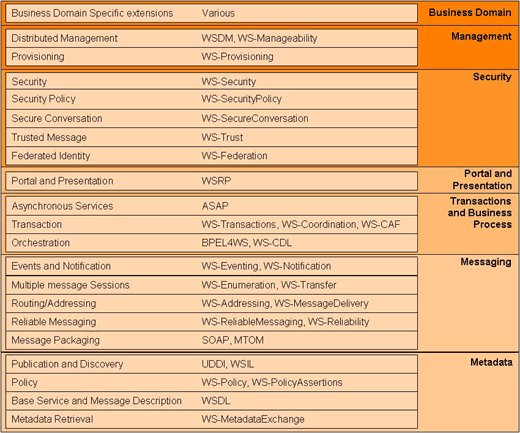
\includegraphics[width=6cm]{images/ws-stack}
\caption{Pila de tecnologías para Servicios Web.}

\end{figure}

}



\frame{
  \frametitle{Servicios} 
\begin{exampleblock}{Proceso de
negocio~\cite{JuricBPEL2006,IBMBPEL2007}}
Un proceso de negocio es una colección de invocaciones coordinadas a
distintos servicios que produce un resultado de negocio, bien dentro de una
organización o través de varias.
\end{exampleblock}

\begin{block}{BPM}
\begin{itemize}
 \item \textit{Business Process Management}.
\item \textit{Business Process Modelling}.
\item \textit{Business Process Modeling Notation}.
\end{itemize}

\end{block}

}


\frame{
  \frametitle{Servicios} 
\begin{exampleblock}{BPEL}
BPEL, convergencia de WSFL (\textit{Web Services Flow Language} de IBM) y XLANG
(Microsof) surge como solución estándar y general  para la composición de
servicios web en procesos de negocio y para exponer la funcionalidad de las
aplicaciones como servicios. Última versión 2.0 (WS-BPEL 2.0) (\textbf{estándar}
de
OASIS). 
\end{exampleblock}


}

\frame{
  \frametitle{Servicios} 
\begin{block}{Características BPEL}
\begin{itemize}
\item Descripción de la lógica de negocio a través de la composición de
servicios.
\item Composición de grandes procesos de negocios mediante la combinación de
servicios y procesos más pequeños.
\item Manejo síncrono y asíncrono de las invocaciones y respuestas.
\item Invocación a los servicios en secuencia o en paralelo.
\item Posibilidad de realizar operaciones de compensación en caso de fallos.
\item Soporte para transacciones.
\item Monitorización de las actividades realizadas.
\end{itemize}
\end{block}

}

\frame{
  \frametitle{Servicios} 
\begin{exampleblock}{Implementaciones BPEL}
\begin{itemize}
\item \textit{Open source}: ActiveBPEL, Apache ODE o Apache
Agila.
\item Comerciales como: OracleBPEL, Microsoft BizTalk, IBM \textit{WebSphere
Business
Integration Server Foundation}, BEA \textit{WebLogic Integration} relacionado
con AquaLogic o JBPM de JBoss. 
\end{itemize}
\end{exampleblock}

}




\frame{
  \frametitle{Infraestructura} 
\begin{exampleblock}{Infraestructura}<1->
Los \textit{Entreprise Service Bus} (ESB), son considerados como la
pieza clave para la integración en arquitecturas empresariales.


\textit{The Enterprise Service Bus is a simple way to do integration within a
Service.}
\end{exampleblock}

\begin{block}{Ejemplos}<2->
IBM, Tibco~\footnote{\url{http://www.tibco.es/}}
Microsoft, Oracle, JBoss~\footnote{\url{http://jboss.org/jbossesb/}},
Mule~\footnote{\url{http://www.mulesource.org/display/COMMUNITY/Home}}, etc.
\end{block}

}

\frame{
  \frametitle{Infraestructura} 




\begin{columns}[c] % the "c" option specifies center vertical alignment
\column{.5\textwidth} % column designated by a command


\begin{exampleblock}{ESB I}<1->



\begin{itemize}
 \item Transparencia de localización.
\item Conversión entre protocolos.
\item  Transformación de mensajes.
\end{itemize}

\end{exampleblock}


\column{.5\textwidth}


\begin{block}{ESB II}<2->
\begin{itemize}
 \item Encaminamiento de mensajes.
\item Enriquecimiento de mensajes.
\item Seguridad. 
\item Monitorización y gestión.
\end{itemize}

\end{block}

\end{columns}

}


\frame{
  \frametitle{Infraestructura} 
\begin{exampleblock}{Beneficios ESB}

\begin{itemize}[<+->]
\item Integración de aplicaciones.
\item Entorno Heterogéneo homogeneizado.
\item Reducción de coste en la creación de nuevas aplicaciones.
\end{itemize}

\end{exampleblock}

}



\frame{
  \frametitle{SOA} 
Por qué adoptar este paradigma~\footnote{Informe de Gartner: ``Justifying
Service-Oriented Architecture Initiatives'', 13 Abril de 2007. ID Number:
G00147984.
}\footnote{Informe de Gartner: ``Service-Oriented Architecture Overview and
Guide
to SOA Research'', 3 Enero de 2008. ID Number: G00154463.
} ...

\begin{figure}[htb]
\centering
	
\includegraphics[width=2cm]{images/marketing}
\caption{SOA estrategia.}

\end{figure}

}


\frame{
  \frametitle{SOA} 
\begin{exampleblock}{Ventajas SOA, provee:}
\begin{itemize}
\item Una forma estandarizada de despliegue y acceso a las aplicaciones.
\item Una infraestructura de comunicaciones común basada en bus.
\item Una arquitectura integrada: nuevos servicios y existentes.
\item Un lenguaje común y estándar para la creación procesos de negocio.
\item Un modelo de despliegue de nuevas soluciones de forma rápida y sencilla.
\end{itemize}
\end{exampleblock}

\begin{block}{Efectos colaterales}
 Reducción de costes y rentabilidad de la inversión.
\end{block}


}

\frame{
  \frametitle{SOA} 
\begin{alertblock}{...pero...}
\begin{itemize}
\item El esfuerzo inicial es muy duro.
\item Es difícil poner de acuerdo a las partes (integración).
\item Complicaciones con la compatibilidad hacia atrás (interoperabilidad).
\item El conocimiento reside en los programadores.
\item Ausencia de buena documentación
\item \ldots
\end{itemize}
\end{alertblock}

}


\subsection{SOA+Semántica}

\frame{
  \frametitle{SOA+Semántica} 
\begin{block}{Dos líneas}
\begin{enumerate}[<+->]
\item Formalización del conocimiento. Modelos de conocimiento compartido en un
dominio (MCD).
\item Servicios web semánticos (SWS).
\end{enumerate}
\end{block}

}

\frame{
  \frametitle{MCD} 

\begin{exampleblock}{Modelo Conceptual de Dominio}
 Modelo semántico sobre un dominio de negocio concreto. Sistema de conocimiento
que describe las entidades y propiedades, así como las relaciones lógicas que
existen entre ellas.
\end{exampleblock}


}

\frame{
  \frametitle{MCD} 

\begin{exampleblock}{Construcción}
\begin{itemize}[<+->]
 \item RDF (W3C Recommendation 10 February 2004). El
\textit{Resource Description Framework} es el modelo de datos básico para la Web
 semántica. Grafo dirigido etiquetado, donde nodos y
arcos están etiquetados mediante URIs (\textit{Uniform Resource Identifier}).

\item RDFS (W3C Recommendation 10 February 2004). El RDF
Vocabulary
Description Language 1.0 o RDF Schema es una extensión de RDF
para la construcción de vocabularios y terminologías en la Web Semántica. Tiene
un sistema de tipos básico:
\begin{itemize}
 \item \textit{rdfs:Class}, \textit{rdfs:Property}, \textit{rdfs:subClassOf},
\textit{rdfs:subPropertyOf}, \textit{rdfs:domain} y \textit{rdfs:range}.
\end {itemize}

\end{itemize}

\end{exampleblock}


}

\frame{
  \frametitle{MCD} 

\begin{exampleblock}{Construcción-II}
\begin{itemize}[<+->]
\item OWL (W3C Recommendation 10 February 2004). Es la
recomendación
del W3C 
para la construcción de ontologías en la Web Semántica. OWL es en realidad una
familia de tres lenguajes con diferente nivel
de expresividad: OWL-Lite, OWL-DL y OWL-Full. OWL-DL. Última versión OWL 2.0.
\item WSML (\textit{Web Service Modelling Language}). Es
una familia de lenguajes resultante de varios proyectos europeos y dentro de la
iniciativa WSMO (\textit{Web Service Modeling Ontology}) para la introducción de
semántica en arquitecturas orientadas a servicios. 

\end{itemize}

\end{exampleblock}


}


\frame{
  \frametitle{MCD} 

\begin{exampleblock}{Construcción-III}
\begin{itemize}
\item
RIF~\footnote{\url{http://www.w3.org/2005/rules/Overview.html}}(\textit{Rule
Interchange Format}).

\item SCOR Model~\footnote{\url{
http://www.supply-chain.org/cs/root/scor_tools_resources/scor_model/scor_model}}
(\textit{Supply-Chain Operations Referente-Model}).

\item SBVR~\footnote{\url{http://www.businessrulesgroup.org/sbvr.shtml}}
(\textit{Semantics of Business Vocabulary and Business Rules}).

\item Clasificaciones de productos de comercio
electrónico.

\item ebXML-\textit{Electronic Business using eXtensible Markup
Language}~\footnote{\url{http://www.ebxml.org/}}.


\item XBRL~\footnote{\url{http://www.xbrl.es/}} (\textit{extensible Business
Reporting Language}).


\end{itemize}

\end{exampleblock}


}



\frame{
  \frametitle{MCD} 

\begin{exampleblock}{Ventajas}
\begin{itemize}
 \item Definición formal de las entidades y relaciones de un dominio.
\item Modelo de datos unificado.
\item Estandarización de un sector. Modelo consensuado.
\item Mejora la documentación y conocimiento del sector.
\end{itemize}

\end{exampleblock}


}




\frame{
  \frametitle{SWS} 

\begin{block}{Tres enfoques}
\begin{enumerate}[<+->]
\item Anotaciones en los servicios.
\item Creación de una plataforma completa (SWS), \textit{full semantics}.
\item Reutilización de plataformas (Semántica+SOA), \textit{partial semantics}.
\end{enumerate}
\end{block}


}


\frame{
  \frametitle{SWS} 


\begin{figure}[htb]
\centering
	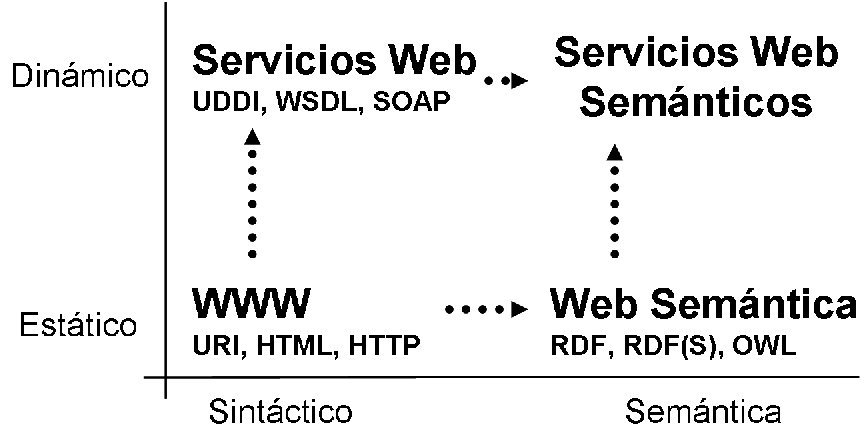
\includegraphics[width=8cm]{images/sws}
\caption{Servicios Web Semánticos (idealmente).}

\end{figure}

}


\frame{
  \frametitle{SWS}

\begin{block}{...son~\cite{BursteinBZFHPSW}...}<1->
Una solución integrada para la siguiente generación web. 
\end{block}

\begin{exampleblock}{Conjunción de tecnología:}<1->
 \begin{itemize}
  \item Web semántica (formalización del conocimiento mediante ontologías +
información procesable automáticamente por las máquinas).
\item Servicios web actuales (descubrimiento automático, selección, composición,
etc.).
 \end{itemize}

\end{exampleblock}

}





\frame{
  \frametitle{SWS} 

\begin{block}{1-Anotaciones en los servicios}
\begin{itemize}[<+->]

\item WSDL-S (W3C Member Submission 7 November 2005). Anotación
semántica de los elementos definidos dentro del
interfaz de la descripción del servicio web. Se aprovecha de las propiedades de
extensibilidad de WSDL (1.1 y 2.0).

\item SAWSDL (W3C Recommendation 28 August 2007). \textit{Semantic
Annotations} para WSDL y XML Schema es una  propuesta define cómo añadir
anotaciones semánticas a diferentes partes de un documento WSDL: mensajes,
interfaces y operaciones.
\begin{itemize}
\item \texttt{sawsdl:modelReference}, relación con el modelo.
\item \texttt{sawsdl:lifting SchemaMapping} y
\item \texttt{sawsdl:lowering SchemaMapping}  para el \textit{grounding}.
\end{itemize}

\end{itemize}
\end{block}


}


\frame{
  \frametitle{SWS} 

\begin{block}{2-Plataformas Completas (\textit{full semantics})}
\begin{itemize}[<+->]
\item SWSF (W3C Member Submission 9 September 2005).
\textit{Semantic Web
Service Framework} es una propuesta que ha sido realizada por el grupo de
trabajo
\textit{W3C Semantic Web Service Initiative} (SWSI). Define ontologías y reglas.

\item OWL-S (W3C Member Submission 22 November 2004). Esta
propuesta tiene su base en la tecnología desarrollada previamente en el proyecto
DAML-S de la agencia DARPA y del cual han surgido entre otros el lenguaje web
W3C  recomendación para la construcción de ontologías, OWL.

\item \textit{OASIS Semantic Execution Environment}. Grupo de OASIS
encargado del desarrollo de guías, justificaciones e implementaciones de
referencia para el despliegue de servicios web semánticos en SOA.
\end{itemize}
\end{block}


}


\frame{
  \frametitle{SWS} 


\begin{figure}[htb]
\centering
	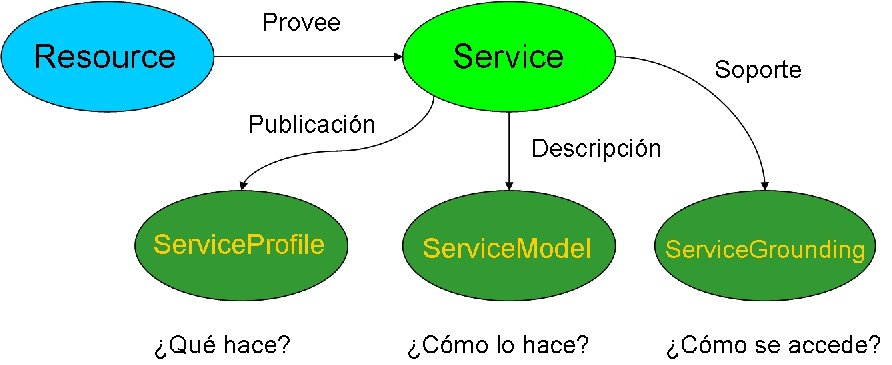
\includegraphics[width=8cm]{images/owl-s}
\caption{OWL-S.}

\end{figure}

}



\frame{
  \frametitle{SWS} 

\begin{block}{2-Plataformas Completas (\textit{full semantics})}
\begin{itemize}[<+->]
\item WSMO (W3C Member Submission 3 June 2005). \textit{Web Service
Modeling Ontology} es una propuesta que nace con el objetivo de especificar
todos los aspectos relevantes en los servicios web semánticos.
\begin{itemize}
\item Ontología WSMO.
\item Lenguaje para ontologías WSML (DL, FOL, RULE y Lite).
\item Entorno de ejecución WSMX.
\item Entorno de desarrollo WSMT.
\end{itemize}
\end{itemize}
\end{block}


}



\frame{
  \frametitle{SWS} 

\begin{exampleblock}{Elementos de WSMO}
\begin{itemize}[<+->]
\item \textit{Ontology}.
\item \textit{Web Service}.
\item \textit{Goal}.
\item \textit{Mediator}.
\end{itemize}
\end{exampleblock}


}








\frame{
  \frametitle{SWS} 

\begin{block}{Implementaciones}
\begin{itemize}

\item<1-> Meteor-S (para WSDL-S).
\item<2-> OWL-S \textit{Virtual Machine}.
\item<3-> WSMX (para WSMO).
\item<3-> IRS-III (para WSMO).
\end{itemize}
\end{block}

}

\frame{
  \frametitle{SWS} 


\begin{figure}[htb]
\centering
	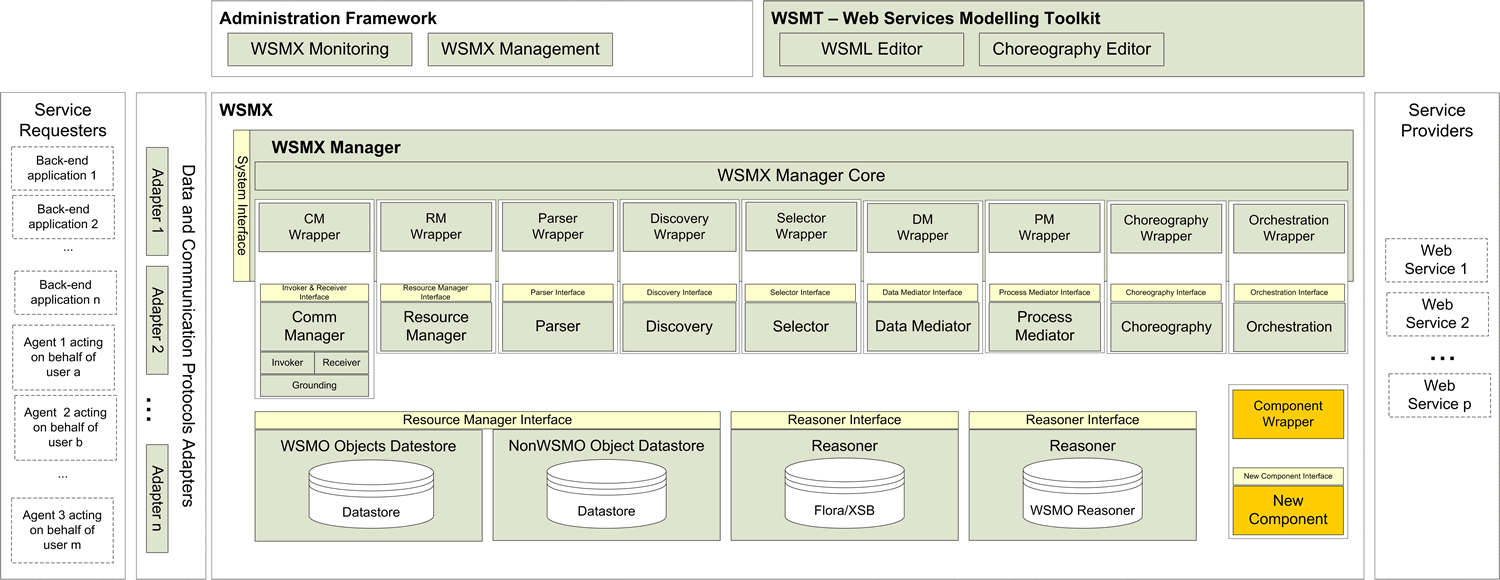
\includegraphics[width=8cm]{images/wsmx}
\caption{Arquitectura de WSMX.}
\label{fig:wsmx}
\end{figure}

}


\frame{
  \frametitle{SWS} 

\begin{block}{3-Plataformas Parciales (\textit{partial semantics})}
\begin{itemize}[<+->]
\item Astro Project. Semántica para verificar, supervisar y sintetizar los
servicios. Descripción de los servicios con tecnologías como OWL-S o WSMO.
Aspira a la composición de servicios con semántica para conseguir procesos
ejecutables.
\item SUPER Project~\footnote{\url{http://www.ip-super.org/}}. Es un proyecto
que ha extendido, entre otras cosas, el ESB de Apache ODE y el lenguaje BPEL
para añadir semántica.
\item SOA4All Project~\footnote{\url{http://www.soa4all.eu/}}. Conjuga la
experiencia de anteriores proyectos (WSMO) para obtener un
capa de servicios completa.
\end{itemize}
\end{block}


}



\frame{
  \frametitle{SWS} 

¿Evaluación?

\begin{figure}[htb]
\centering
	
\includegraphics[width=4cm]{images/evaluation}
\caption{Evaluación.}

\end{figure}


}


\frame{
  \frametitle{SWS} 

\begin{block}{Evaluación}
\begin{itemize}[<1->]
\item Muchos proyectos de investigación.
\item Muchos enfoques.
\item Muchas especificaciones, guías, \textit{papers}, \textit{lobby}, etc. 
\item Mucha inversión.
\end{itemize}
\end{block}

}


\frame{
  \frametitle{SWS} 




\begin{columns}[c] % the "c" option specifies center vertical alignment
\column{.5\textwidth} % column designated by a command


\begin{figure}[htb]
\centering
	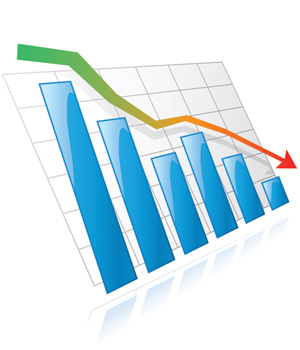
\includegraphics[width=3cm]{images/mal-eval}
\caption{Evaluación a la baja.}

\end{figure}

\column{.5\textwidth}


\begin{alertblock}{...pero...}
\begin{itemize}
\item Poco retorno.
\item Especificaciones y plataformas de ejecución incompletas.
\item Lejos de salir del laboratorio.
\item Falta de reutilización: trabajos, estándares, etc.
\end{itemize}
\end{alertblock}

\end{columns}

}

\frame{
  \frametitle{SWS} 

\begin{exampleblock}{Lecciones aprendidas}<1->
\begin{itemize}
\item Anotar servicios con un MCD.
\item Centrar esfuerzos. No constuir plataformas desde 0.
\item Utilizar estándares.
\item Delegar ejecución.
\end{itemize}
\end{exampleblock}

\begin{alertblock}{...}<2->
 Mejor hablar de semántica aplicada a SOA y no de SWS.
\end{alertblock}


}

